\subsection{Доверительные интервалы для параметров нормального распределения. Асимптотический подход}
    \begin{figure}[H]
		\centering
		    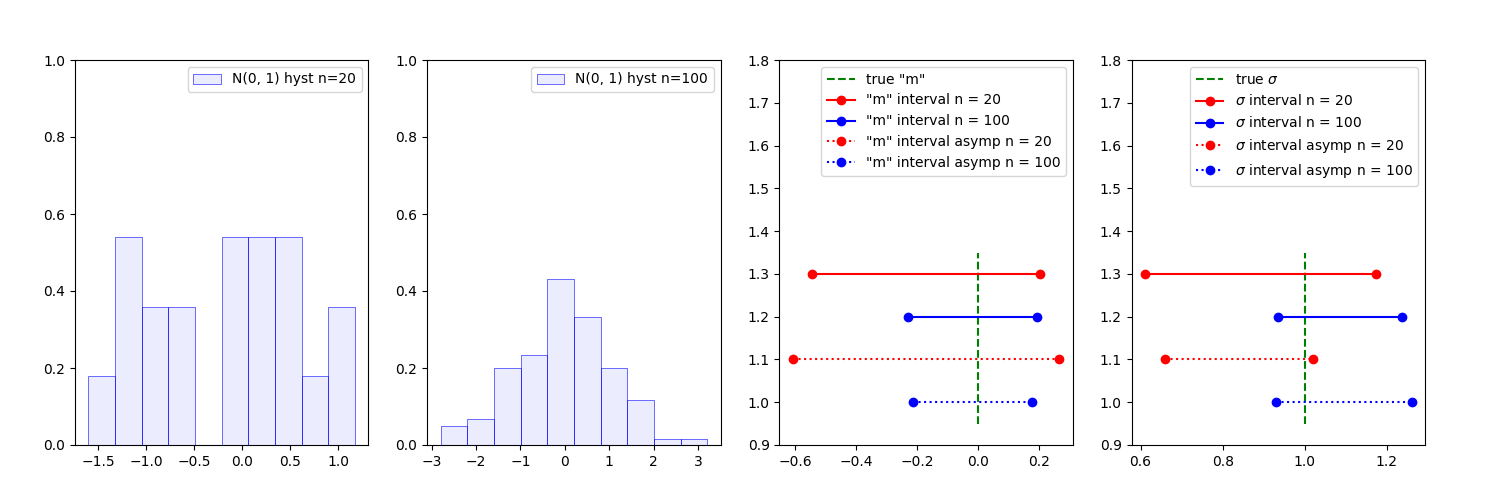
\includegraphics[width = 15cm, height = 5cm]{part_asymp_normal_estimates/figures/norm_asymp}
		\caption{Гистограммы нормальных распределений и доверительные интервалы их параметров}
		\label{fig:hist_norm_estimates}
	\end{figure}

	\begin{table}[H]
	    \centering
	    \begin{tabular}{| c | c | c |}
	    \hline
	       n = 20   &  $m$  & $\sigma$\\ \hline
	          &  -0.57 < $m$ < 0.58 & 0.93 < $\sigma$ < 1.78 \\ \hline
	         &   &   \\ \hline
	       n = 100   &  $m$  & $\sigma$\\ \hline
	        & -0.16 < $m$ < 0.19 & 0.78 < $\sigma$ < 1.03 \\
	   \hline
	    \end{tabular}
	    \caption{Доверительные интервалы для параметров нормального распределения}
	    \label{tab:interv_simple}
	\end{table}

	\begin{table}[H]
	    \centering
	    \begin{tabular}{| c | c | c |}
	    \hline
	       n = 20   &  $m$  & $\sigma$\\ \hline
	          &  -0.43 < $m$ < 0.44 & 0.94 < $\sigma$ < 1.91 \\ \hline
	         &   &   \\ \hline
	       n = 100   &  $m$  & $\sigma$\\ \hline
	        & -0.18 < $m$ < 0.21 & 0.80 < $\sigma$ < 1.01 \\
	   \hline
	    \end{tabular}
	    \caption{Доверительные интервалы для параметров произвольного распределения. Асимптотический подход}
	    \label{tab:interv_asimpt}
	\end{table}